\documentclass[letter,11pt]{article}

\usepackage[spanish,es-nodecimaldot]{babel}
\usepackage[utf8]{inputenc}

\usepackage{lmodern}
\usepackage[T1]{fontenc}
\usepackage{textcomp}

\usepackage{framed}
\usepackage[svgnames]{xcolor}
\colorlet{shadecolor}{Gainsboro!50}

\usepackage{graphicx}
\usepackage{pstricks}

\usepackage{anysize}
\marginsize{3cm}{2cm}{2cm}{3cm}

\usepackage{siunitx}
\usepackage{amsmath}
\usepackage{array}
\usepackage{alltt}

\usepackage{fancyhdr}
\usepackage{lastpage}
\pagestyle{fancy}
\fancyhf{}
\fancyhead[LE,RO]{Dinámica}
\fancyfoot[CO,CE]{\thepage\ de~\pageref{LastPage}}

\special{papersize=215.9mm,279.4mm}

\usepackage[
    pdfauthor={Carlos Eduardo Caballero Burgoa},%
    pdftitle={Dinámica},%
    pdfsubject={Segundo Examen},%
    colorlinks,%
    citecolor=black,%
    filecolor=black,%
    linkcolor=black,%
    urlcolor=black,
    breaklinks]{hyperref}
\usepackage{breakurl}

\newcommand{\blankpage}{
\newpage
\thispagestyle{empty}
\mbox{}
\newpage
}

\renewcommand{\arraystretch}{1.2}

\begin{document}

\begin{center}
    {\large \bf{2do Examen}}
\end{center}

\noindent\fbox{%
    \parbox{\textwidth}{%
        Estudiante: CABALLERO BURGOA, Carlos Eduardo \\
        Carrera: Ingeniería Electromecánica
    }%
}

\vspace{1.0cm}

1. Un péndulo simple de longitud $L$ y peso $mg$ esta pivotando a la masa $M$,
la cual se desliza sin fricción sobre un plano horizontal, como se muestra en la
figura. Utilice la ecuación de \emph{Lagrange} para determinar las ecuaciones de
movimiento del sistema.\\

%\begin{figure}[!h]
%\centering
%\includegraphics[scale=0.5]{resources/tarea_01.eps}
%\end{figure}

\textbf{Solución}: \\

(a) \\

Calculando la energía cinética en coordenadas polares:

\begin{equation*}
    \begin{cases}
        x=r\cos(\theta)\\
        y=r\sen(\theta)
    \end{cases}
\end{equation*}

\begin{equation*}
    \dot{x}=\dot{r}\cos(\theta)-r\sen(\theta)\dot{\theta}
\end{equation*}
\begin{equation*}
    \dot{y}=\dot{r}\sen(\theta)+r\cos(\theta)\dot{\theta}
\end{equation*}

\begin{equation*}
    \dot{x}^2=\dot{r}^2\cos^2(\theta)
             -2\dot{r}r\dot{\theta}\cos(\theta)\sen(\theta)
             +r^2\dot{\theta}^2\sen^2(\theta)
\end{equation*}
\begin{equation*}
    \dot{y}^2=\dot{r}^2\sen^2(\theta)
             +2\dot{r}r\dot{\theta}\sen(\theta)\cos(\theta)
             +r^2\dot{\theta}^2\cos^2(\theta)
\end{equation*}

\begin{equation*}
\begin{split}
    T&=\frac{1}{2}m(\dot{x}^2+\dot{y}^2)\\
     &=\frac{1}{2}m(
           \dot{r}^2\cos^2(\theta)+
           r^2\dot{\theta}^2\sen^2(\theta)+
           \dot{r}^2\sen^2(\theta)+
           r^2\dot{\theta}^2\cos^2(\theta)
       )\\
     &=\frac{1}{2}m(
           \dot{r}^2(
               \cos^2(\theta)+\sen^2(\theta)
           )+
           r^2\dot{\theta}^2(
               \sen^2(\theta)+\cos^2(\theta)
           )
       )\\
     &=\frac{1}{2}m(\dot{r}^2+r^2\dot{\theta}^2)
\end{split}
\end{equation*}

\begin{equation}
\boxed{\begin{array}{l}
    T=\dfrac{1}{2}m(\dot{r}^2+r^2\dot{\theta}^2)
\end{array}}
\label{ec01}
\end{equation}

Calculando las ecuaciones de movimiento:

\begin{equation*}
    \frac{\partial T}{\partial \dot{r}}=m\dot{r}
\end{equation*}
\begin{equation*}
    \frac{d}{dt}\left(\frac{\partial T}{\partial \dot{r}}\right)=m\ddot{r}
\end{equation*}
\begin{equation*}
    \frac{\partial T}{\partial r}=mr\dot{\theta}^2
\end{equation*}

\begin{equation*}
    \frac{\partial T}{\partial \dot{\theta}}=mr^2\dot{\theta}
\end{equation*}
\begin{equation*}
    \frac{d}{dt}\left(
        \frac{\partial T}{\partial \dot{\theta}}
    \right)=mr^2\ddot{\theta}+2mr\dot{r}\dot{\theta}
\end{equation*}
\begin{equation*}
    \frac{\partial T}{\partial \theta}=0
\end{equation*}

\begin{equation*}
    F_r=-\frac{GmM}{r^2}
\end{equation*}
\begin{equation*}
    F_{\theta}=0
\end{equation*}

Resultando:

\begin{equation*}
    m\ddot{r}-mr\dot{\theta}^2+\frac{GmM}{r^2}=0
\end{equation*}
\begin{equation}
\boxed{\begin{array}{l}
    \ddot{r}-r\dot{\theta}^2+\dfrac{GM}{r^2}=0
\end{array}}
\label{ec02}
\end{equation}

\begin{equation*}
    mr^2\ddot{\theta}+2mr\dot{r}\dot{\theta}=0
\end{equation*}
\begin{equation}
\boxed{\begin{array}{l}
    r^2\ddot{\theta}+2r\dot{r}\dot{\theta}=0
\end{array}}
\label{ec03}
\end{equation}
\\

(b) \\

De la segunda ecuación de movimiento se tiene:

\begin{equation}
    \frac{d}{dt}(mr^2\dot{\theta})=0
    \label{ec04}
\end{equation}

Por tanto:

\begin{equation*}
\boxed{\begin{array}{l}
    mr^2\dot{\theta}=\text{constante}
\end{array}}
\end{equation*}

Que representa el \textbf{momento angular ($L$)} de la partícula.
\\

(c) \\

Si denominamos $h=L/m$:

\begin{equation}
    \dot{\theta}=\frac{h}{r^2}
    \label{ec05}
\end{equation}

Reemplazando $\dot{\theta}$ en (\ref{ec02}):

\begin{equation*}
    \ddot{r}-r{\left(\frac{h}{r^2}\right)}^2+\frac{GM}{r^2}=0
\end{equation*}
\begin{equation}
    \ddot{r}-\frac{h^2}{r^3}+\frac{GM}{r^2}=0
    \label{ec06}
\end{equation}
\\

Se realizará un cambio de variable:

\begin{equation}
    q=\frac{1}{r}
    \label{ec07}
\end{equation}

Calculamos $\dot{r}$ y $\ddot{r}$, con la ayuda de (\ref{ec05}) y (\ref{ec06}):

\begin{equation*}
    \dot{r}=\frac{dr}{dt}
           =\frac{dr}{d\theta}\frac{d\theta}{dt}
           =\frac{d}{d\theta}\left(\frac{1}{q}\right)\dot{\theta}
           =-\frac{1}{q^2}\frac{dq}{d\theta}\left(\frac{h}{r^2}\right)
           =-\frac{1}{q^2}\frac{dq}{d\theta}(hq^2)
\end{equation*}
\begin{equation}
    \dot{r}=-h\frac{dq}{d\theta}
    \label{ec08}
\end{equation}

\begin{equation*}
    \ddot{r}=\frac{d\dot{r}}{dt}
            =\frac{d\dot{r}}{d\theta}\frac{d\theta}{dt}
            =\frac{d}{d\theta}\left(-h\frac{dq}{d\theta}\right)\dot{\theta}
            =-h\frac{d^2q}{d\theta^2}\left(\frac{h}{r^2}\right)
            =-h\frac{d^2q}{d\theta^2}(hq^2)
\end{equation*}
\begin{equation}
    \ddot{r}=-h^2q^2\frac{d^2q}{d\theta^2}
    \label{ec09}
\end{equation}

Reemplazando (\ref{ec09}) y (\ref{ec07}) en (\ref{ec06}):

\begin{equation*}
    -h^2q^2\frac{d^2q}{d\theta^2}-h^2q^3+GMq^2=0
\end{equation*}
\begin{equation*}
    q^2\left(-h^2\left(\frac{d^2q}{d\theta^2}+q\right)+GM\right)=0
\end{equation*}
\begin{equation}
\boxed{\begin{array}{l}
    \dfrac{d^2q}{d\theta^2}+q=\dfrac{GM}{h^2}
\end{array}}
\label{ec10}
\end{equation}
\\

Ecuación diferencial cuya solución general es:

\begin{equation}
    q(\theta)=A\cos(\theta)+B\sen(\theta)+\frac{GM}{h^2}
    \label{ec11}
\end{equation}
\\

Para calcular los coeficientes $A$ y $B$ se plantean condiciones iniciales:

\begin{itemize}
\item Para $t=0$, $r=r_0$, asumiendo $\theta=0$:
    \begin{equation}
        q(0)=\frac{1}{r_0}
        \label{ec12}
    \end{equation}
\item Para $t=0$, la velocidad radial $\dot{r}=\dot{r}_0$, asumiendo $\theta=0$
y usando la ecuación (\ref{ec08}):
    \begin{equation}
        \frac{dq}{d\theta}(0)=-\frac{\dot{r}_0}{h}
        \label{ec13}
    \end{equation}
\item Para $t=0$, la velocidad angular $\dot{\theta}=\dot{\theta}_0$, y
sustituyendo $h$:
    \begin{equation}
        h=\frac{L}{m}=\frac{mr^2_0\dot{\theta}_0}{m}=r^2_0\dot{\theta}_0
        \label{ec14}
    \end{equation}
\end{itemize}

Reemplazando las condiciones (\ref{ec12}) y (\ref{ec14}) en (\ref{ec11}):

\begin{equation*}
    q(0)=A\cos(0)+B\sen(0)+\frac{GM}{{(r^2_0\dot{\theta}_0)}^2}
\end{equation*}
\begin{equation*}
    \frac{1}{r_0}=A+\frac{GM}{{(r^2_0\dot{\theta}_0)}^2}
\end{equation*}
\begin{equation}
    A=\frac{1}{r_0}-\frac{GM}{{(r^2_0\dot{\theta}_0)}^2}
    \label{ec15}
\end{equation}

Derivando la ecuación (\ref{ec11}) y reemplazando (\ref{ec13}) y (\ref{ec14}):

\begin{equation*}
    \frac{dq(\theta)}{d\theta}=A(-\sen(\theta))+B\cos(\theta)
\end{equation*}
\begin{equation*}
    \frac{dq(0)}{d\theta}=-A\sen(0)+B\cos(0)
\end{equation*}
\begin{equation}
    B=-\frac{\dot{r}_0}{r^2_0\dot{\theta}_0}
    \label{ec16}
\end{equation}
\\

2. Una palanqueta que consiste en dos esferas iguales pequeñas, unidas
rigidamente a los extremos de una varilla delgada y lisa, puede moverse
libremente en el espacio dentro de un fluido viscoso. Sin necesidad de tener en
cuenta la resistencia sobre la varilla y suponiendo que no hay rotación de las
esferas alrededor del eje que coincide con la varilla, determinar la funcion de
potencia $P$.

Suponer que las coordenadas $x$, $y$, $z$, localizan el centro de masa de la
palanqueta, $l$ es la distancia del centro de masa, al cento de una de las
esferas. $\theta$ y $\phi$ son las coordenadas esfericas usuales.
\\

3. Una particula se mueve en contacto con un tablero horizontal rugoso.
Suponiendo que el coeficiente de fricción para movimiento en la dirección de
$X$ es $\mu_x$ y que en la dirección de $Y$ es $\mu_y$. Determinar las fuerzas
de fricción generalizadas, correspondientes a las coordenadas $r$ y $\theta$,
o sea $F_r$ y $F_{\theta}$.

\end{document}

